\chapter{Resultados Experimentales}\label{cap5}
A fin de evaluar empíricamente los algoritmos implementados se han analizado sus comportamientos sobre grafos representados como diagramas de arcos, que fueron generados aleatoriamente. Se utilizó el ``número de nodos" como semilla para la generación aleatoria. Los arcos fueron generados aleatoriamente tanto en la posición de la curva sobre o por debajo del semiplano, como en los nodos que conectan, por lo que para una misma semilla (número de nodos) puede haber una cantidad variable de arcos que conectan diferentes nodos. 

En cada prueba se generaron 100 grafos para cada semilla, es decir 100 grafos aleatorios para cada número de nodos. Los resultados muestran los promedios de arcos generados, de tiempos y ciclos invertidos (para el caso del algoritmo genético) y de valores de crossing number inicial y final para cada semilla. 

En las pruebas mencionadas se utilizaron los mismos grafos aleatorios, es decir que sobre cada grafo original se aplicaron los algoritmos en diferentes ordenes y sucesiones de unos y otros, y de esta manera se pudo comparar el rendimiento de cada uno con respecto a los demás, como se muestra en la sección \ref{sec:resultados_finales}.

Estos resultados fueron obtenidos ejecutando un lote de pruebas sobre una computadora con procesador Intel Core i7-8650 de 2.11GHz, con una memoria RAM de 16GB y bajo un sistema operativo Windows 10 x64.

\section{Resultados de Algoritmo de Grafos Completos}
Esta prueba fue realizada a partir de aplicar el algoritmo para grafos completos, explicado en los capítulos anteriores, sobre un grafo original representado como diagrama de arcos que fue generado aleatoriamente como se explicó en la sección previa. En la figura \ref{fig:resultado_ejemplo_grafo_ori_lin} puede verse un ejemplo de aplicación del algoritmo. En la Tabla \ref{tab:resultados_orig_alg_com} pueden verse los promedios de tiempos de ejecución y de los crossing number resultantes comparados con los de los grafos originales para cada semilla.

\begin{figure*}[h]
	\centering
	\subfigure[Grafo original (CN: 209).]{
		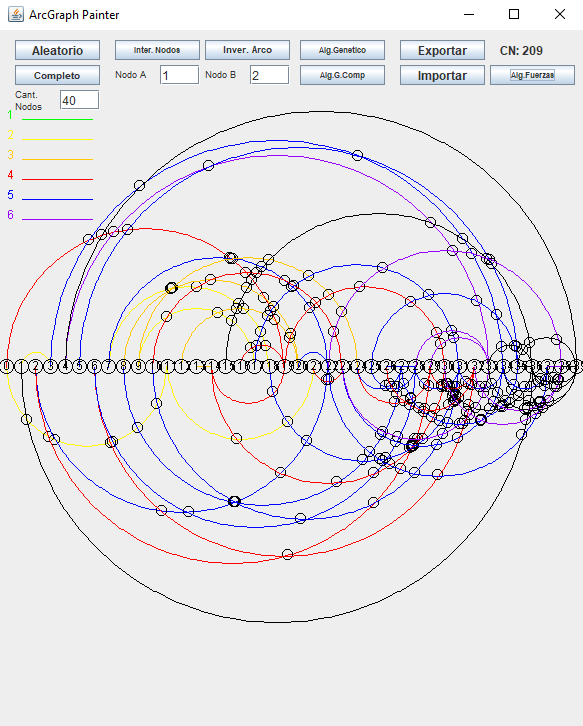
\includegraphics[width=0.45\textwidth]{imagenes/grafo_example_ori.png}
	}
	\subfigure[Grafo luego de aplicar algoritmo para grafos completos (CN: 123).]{
		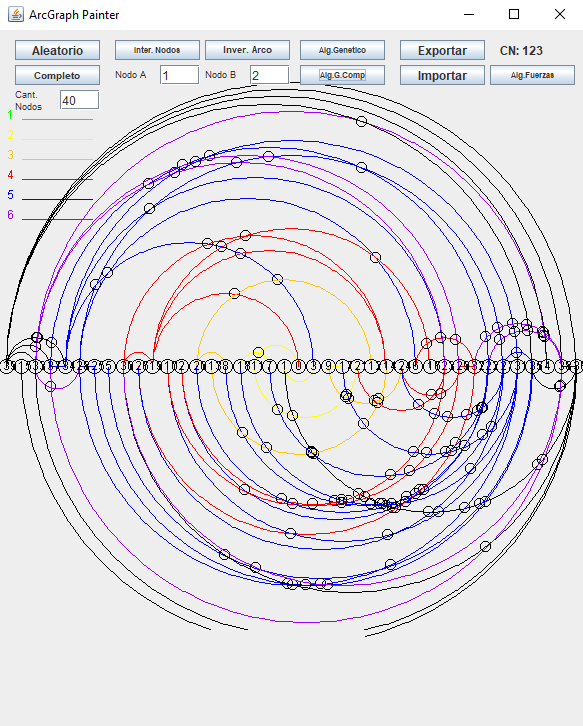
\includegraphics[width=0.45\textwidth]{imagenes/grafo_example_ori_lin.png}
	}
	\caption{Ejemplo de aplicar algoritmo para grafos completos sobre un grafo de 40 nodos aleatorio.}
	\label{fig:resultado_ejemplo_grafo_ori_lin}
\end{figure*}

\begin{table}[H]
	\caption{Promedios de 100 pruebas sobre cada semilla (de 5 a 50), del algoritmo para grafos completos sobre los grafos originales aleatorios.}
	\label{tab:resultados_orig_alg_com}
	\begin{tabularx}{\linewidth}{|p{1.5cm}|p{1.2cm}|p{1.5cm}|X|X|}
		\hline
		\multirow{2}{2cm}{\textbf{Nro. Nodos (semilla)}} & \multicolumn{4}{c|}{\textbf{Promedios}} \\
		\cline{2-5}
		& \textbf{Nro. Arcos} & \textbf{Tiempo} & \textbf{CN Grafo Origininal} & \textbf{CN Grafo Final} \\
		\hline
		10 & 13 & 0.000 s. & 7 & 3 \\
		\hline
		15 & 20 & 0.000 s. & 18 & 10 \\
		\hline
		20 & 28 & 0.001 s. & 38 & 23 \\
		\hline
		25 & 35 & 0.001 s. & 66 & 42 \\
		\hline
		30 & 43 & 0.001 s. & 103 & 63 \\
		\hline
		35 & 50 & 0.001 s. & 139 & 91 \\
		\hline
		40 & 58 & 0.001 s. & 195 & 123 \\
		\hline
		45 & 65 & 0.001 s. & 240 & 161 \\
		\hline
		50 & 73 & 0.002 s. & 312 & 198 \\
		\hline
	\end{tabularx}
\end{table}

\section{Resultados de Algoritmo ArcGen}
En estas pruebas se evalúan los resultados de aplicar el algoritmo genético ArcGen, explicado en los capítulos anteriores, sobre diferentes grafos de entrada.

\subsection{Resultados sobre Grafo Original}
Esta prueba aplica el algoritmo genético ArcGen sobre el grafo original generado aleatoriamente. En la figura \ref{fig:resultado_ejemplo_grafo_ori_gen} puede verse un ejemplo de aplicación del algoritmo. En la Tabla \ref{tab:resultados_orig_alg_gen} pueden verse los promedios de tiempos de ejecución, de las cantidades de ciclos y de los crossing number resultantes comparados con los de los grafos originales para cada semilla.

\begin{figure*}[h]
	\centering
	\subfigure[Grafo original (CN: 209).]{
		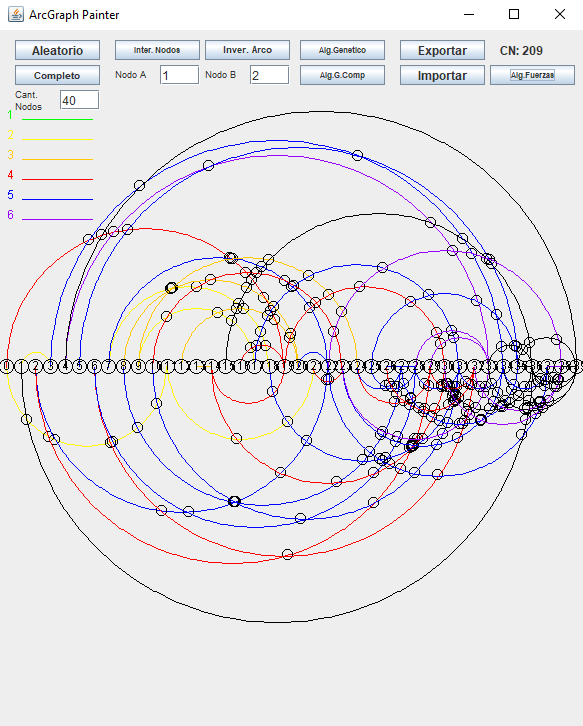
\includegraphics[width=0.45\textwidth]{imagenes/grafo_example_ori.png}
	}
	\subfigure[Grafo luego de aplicar algoritmo ArcGen (CN: 32).]{
		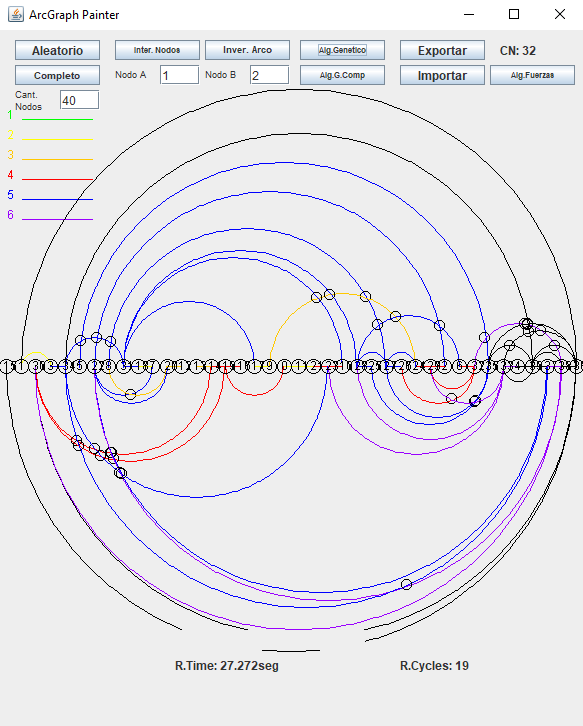
\includegraphics[width=0.45\textwidth]{imagenes/grafo_example_ori_gen.png}
	}
	\caption{Ejemplo de aplicar algoritmo ArcGen sobre un grafo de 40 nodos aleatorio.}
	\label{fig:resultado_ejemplo_grafo_ori_gen}
\end{figure*}

\begin{table}[H]
	\caption{Promedios de 100 pruebas sobre cada semilla (de 5 a 50), del algoritmo genético ArcGen sobre los grafos originales aleatorios.}
	\label{tab:resultados_orig_alg_gen}
	\begin{tabularx}{\linewidth}{|p{1.5cm}|p{1.2cm}|p{1.5cm}|p{1.5cm}|X|X|}
		\hline
		\multirow{2}{2cm}{\textbf{Nro. Nodos (semilla)}} & \multicolumn{5}{c|}{\textbf{Promedios}} \\
		\cline{2-6}
		& \textbf{Nro. Arcos} & \textbf{Tiempo} & \textbf{Ciclos} & \textbf{CN Grafo Original} & \textbf{CN Grafo Final} \\
		\hline
		10 & 13 & 0.024 s. & 2 & 7 & 0 \\
		\hline
		15 & 20 & 0.164 s. & 4 & 18 & 1 \\
		\hline
		20 & 28 & 0.613 s. & 7 & 38 & 4 \\
		\hline
		25 & 35 & 1.809 s. & 10 & 66 & 7 \\
		\hline
		30 & 43 & 10.953 s. & 13 & 103 & 12 \\
		\hline
		35 & 50 & 15.558 s. & 16 & 139 & 19 \\
		\hline
		40 & 58 & 15.921 s. & 20 & 195 & 27 \\
		\hline
		45 & 65 & 23.535 s. & 24 & 240 & 34 \\
		\hline
		50 & 73 & 45.778 s. & 28 & 312 & 43 \\
		\hline
	\end{tabularx}
\end{table}

\subsection{Resultados sobre Grafo Preprocesado por Algoritmo de Grafos Completos}
Esta prueba aplica el algoritmo genético ArcGen sobre el grafo original (generado aleatoriamente), luego de ser preprocesado por el algoritmo para grafos completos. En la figura \ref{fig:resultado_ejemplo_grafo_ori_lin_gen} puede verse un ejemplo de aplicación del algoritmo. En la Tabla \ref{tab:resultados_com_alg_gen} pueden verse los promedios de tiempos de ejecución, de las cantidades de ciclos y de los crossing number resultantes comparados con los de los grafos preprocesados para cada semilla.

\begin{figure*}[h]
	\centering
	\subfigure[Grafo preprocesado por algoritmo para grafos completos (CN: 123).]{
		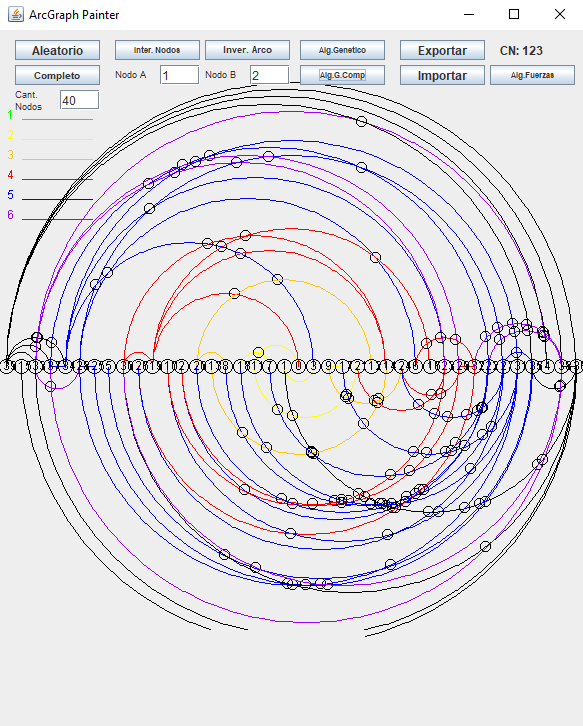
\includegraphics[width=0.45\textwidth]{imagenes/grafo_example_ori_lin.png}
	}
	\subfigure[Grafo luego de aplicar algoritmo ArcGen (CN: 39).]{
		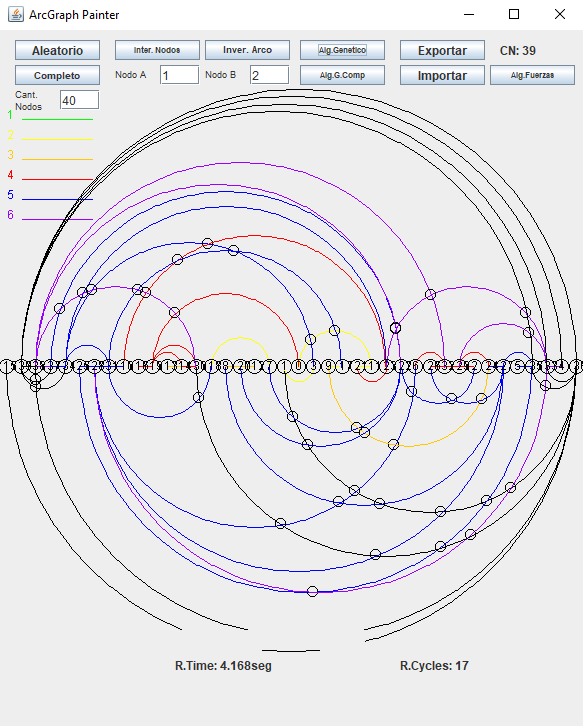
\includegraphics[width=0.45\textwidth]{imagenes/grafo_example_ori_lin_gen.png}
	}
	\caption{Ejemplo de aplicar algoritmo ArcGen sobre un grafo de 40 nodos aleatorio preprocesado por el algoritmo para grafos completos.}
	\label{fig:resultado_ejemplo_grafo_ori_lin_gen}
\end{figure*}

\begin{table}[H]
	\caption{Promedios de 100 pruebas sobre cada semilla (de 5 a 50), del algoritmo genético ArcGen sobre los grafos originales aleatorios preprocesados por el algoritmo para grafos completos.}
	\label{tab:resultados_com_alg_gen}
	\begin{tabularx}{\linewidth}{|p{1.5cm}|p{1.2cm}|p{1.5cm}|p{1.5cm}|X|X|}
		\hline
		\multirow{2}{2cm}{\textbf{Nro. Nodos (semilla)}} & \multicolumn{5}{c|}{\textbf{Promedios}} \\
		\cline{2-6}
		& \textbf{Nro. Arcos} & \textbf{Tiempo} & \textbf{Ciclos} & \textbf{CN Grafo Preprocesado} & \textbf{CN Grafo Final} \\
		\hline
		10 & 13 & 0.002 s. & 2 & 3 & 0 \\
		\hline
		15 & 20 & 0.023 s. & 4 & 10 & 1 \\
		\hline
		20 & 28 & 0.084 s. & 6 & 23 & 4 \\
		\hline
		25 & 35 & 0.308 s. & 9 & 42 & 8 \\
		\hline
		30 & 43 & 1.765 s. & 12 & 63 & 13 \\
		\hline
		35 & 50 & 2.757 s. & 14 & 91 & 20 \\
		\hline
		40 & 58 & 3.202 s. & 18 & 123 & 30 \\
		\hline
		45 & 65 & 6.152 s. & 21 & 161 & 39 \\
		\hline
		50 & 73 & 10.885 s. & 25 & 198 & 49 \\
		\hline
	\end{tabularx}
\end{table}

Dados los resultados de las tablas \ref{tab:resultados_orig_alg_gen} y \ref{tab:resultados_com_alg_gen} encontramos que el algoritmo ArcGen aplicado sobre el grafo preprocesado logra alcanzar un máximo local mucho más rápido que al aplicarse sobre el grafo original, pero a coste de que el máximo alcanzado sea menos óptimo.

\section{Resultados de Algoritmo de Fuerzas}
En estas pruebas se evalúan los resultados de aplicar el algoritmo dirigido por fuerzas de Tunkelang, sobre diferentes grafos de entrada.

\subsection{Resultados sobre Grafo Original}
Esta prueba aplica el algoritmo dirigido por fuerzas de Tunkelang sobre el grafo original generado aleatoriamente. En la figura \ref{fig:resultado_ejemplo_grafo_ori_fue} puede verse un ejemplo de aplicación del algoritmo. En la Tabla \ref{tab:resultados_orig_alg_fue} pueden verse los promedios de tiempos de ejecución y de los crossing number resultantes comparados con los de los grafos originales para cada semilla.

\begin{figure*}[h]
	\centering
	\subfigure[Grafo original (CN: 209).]{
		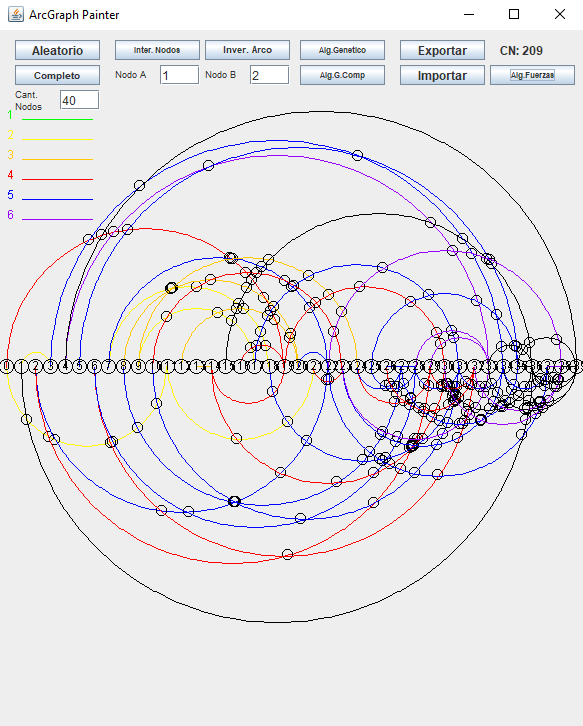
\includegraphics[width=0.45\textwidth]{imagenes/grafo_example_ori.png}
	}
	\subfigure[Grafo luego de aplicar algoritmo dirigido por fuerzas de Tunkelang (CN: 61).]{
		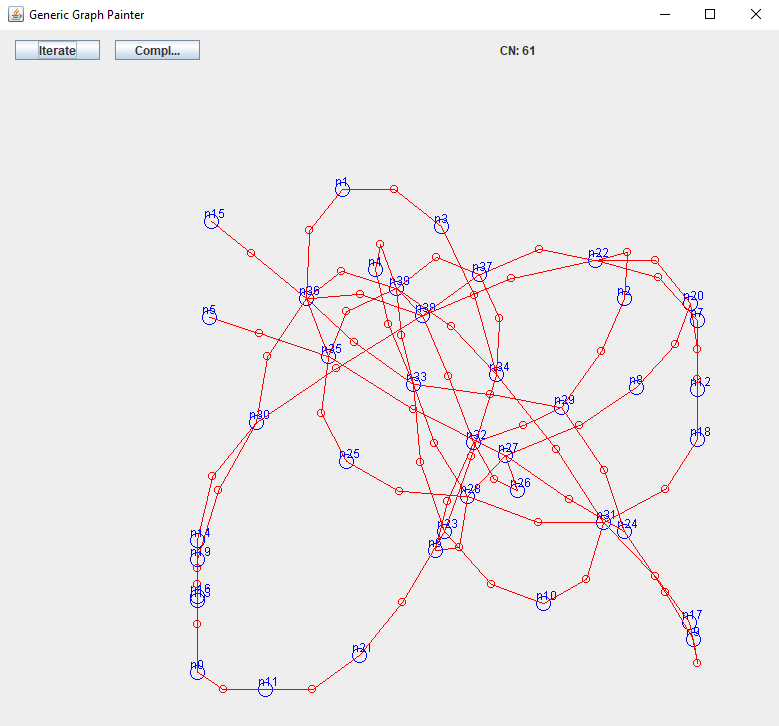
\includegraphics[width=0.5\textwidth]{imagenes/grafo_example_ori_fue.png}
	}
	\caption{Ejemplo de aplicar algoritmo dirigido por fuerzas de Tunkelang sobre un grafo de 40 nodos aleatorio.}
	\label{fig:resultado_ejemplo_grafo_ori_fue}
\end{figure*}

\begin{table}[H]
	\caption{Promedios de 100 pruebas sobre cada semilla (de 5 a 50), del algoritmo dirigido por fuerzas de Tunkelang sobre los grafos originales aleatorios.}
	\label{tab:resultados_orig_alg_fue}
	\begin{tabularx}{\linewidth}{|p{1.5cm}|p{1.2cm}|p{1.5cm}|X|X|}
		\hline
		\multirow{2}{2cm}{\textbf{Nro. Nodos (semilla)}} & \multicolumn{4}{c|}{\textbf{Promedios}} \\
		\cline{2-5}
		& \textbf{Nro. Arcos} & \textbf{Tiempo} & \textbf{CN Grafo Original} & \textbf{CN Grafo Final} \\
		\hline
		10 & 13 & 2.555 s. & 7 & 1 \\
		\hline
		15 & 20 & 2.525 s. & 18 & 3 \\
		\hline
		20 & 28 & 2.539 s. & 38 & 6 \\
		\hline
		25 & 35 & 2.546 s. & 66 & 10 \\
		\hline
		30 & 43 & 2.588 s. & 103 & 17 \\
		\hline
		35 & 50 & 2.593 s. & 139 & 24 \\
		\hline
		40 & 58 & 2.541 s. & 195 & 32 \\
		\hline
		45 & 65 & 2.527 s. & 240 & 42 \\
		\hline
		50 & 73 & 2.531 s. & 312 & 52 \\
		\hline
	\end{tabularx}
\end{table}

\subsection{Resultados sobre Grafo Preprocesado por Algoritmo de Grafos Completos}
Esta prueba aplica el algoritmo dirigido por fuerzas de Tunkelang sobre el grafo original (generado aleatoriamente), luego de ser preprocesado por el algoritmo para grafos completos. En la figura \ref{fig:resultado_ejemplo_grafo_ori_lin_fue} puede verse un ejemplo de aplicación del algoritmo. En la Tabla \ref{tab:resultados_com_alg_fue} pueden verse los promedios de tiempos de ejecución y de los crossing number resultantes comparados con los de los grafos preprocesados para cada semilla.

\begin{figure*}[h]
	\centering
	\subfigure[Grafo preprocesado por algoritmo para grafos completos (CN: 123).]{
		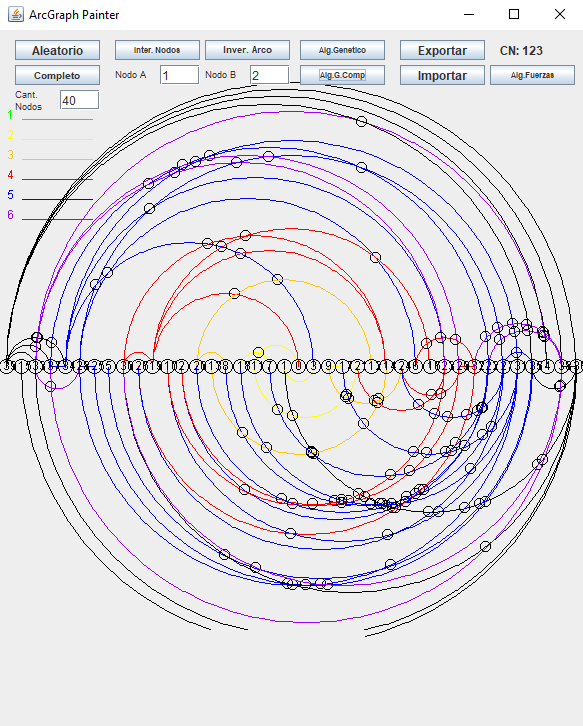
\includegraphics[width=0.45\textwidth]{imagenes/grafo_example_ori_lin.png}
	}
	\subfigure[Grafo luego de aplicar algoritmo dirigido por fuerzas de Tunkelang (CN: 49).]{
		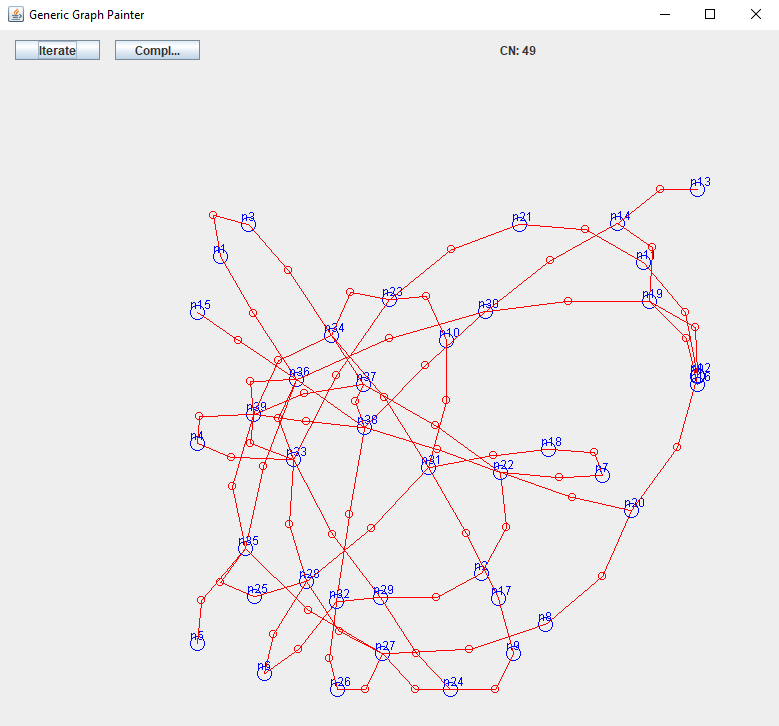
\includegraphics[width=0.5\textwidth]{imagenes/grafo_example_ori_lin_fue.png}
	}
	\caption{Ejemplo de aplicar algoritmo dirigido por fuerzas de Tunkelang sobre un grafo de 40 nodos aleatorio preprocesado por el algoritmo para grafos completos.}
	\label{fig:resultado_ejemplo_grafo_ori_lin_fue}
\end{figure*}

\begin{table}[H]
	\caption{Promedios de 100 pruebas sobre cada semilla (de 5 a 50), del algoritmo dirigido por fuerzas de Tunkelang sobre los grafos originales aleatorios preprocesados por el algoritmo para grafos completos.}
	\label{tab:resultados_com_alg_fue}
	\begin{tabularx}{\linewidth}{|p{1.5cm}|p{1.2cm}|p{1.5cm}|X|X|}
		\hline
		\multirow{2}{2cm}{\textbf{Nro. Nodos (semilla)}} & \multicolumn{4}{c|}{\textbf{Promedios}} \\
		\cline{2-5}
		& \textbf{Nro. Arcos} & \textbf{Tiempo} & \textbf{CN Grafo Preprocesado} & \textbf{CN Grafo Final} \\
		\hline
		10 & 13 & 2.557 s. & 3 & 0 \\
		\hline
		15 & 20 & 2.527 s. & 10 & 2 \\
		\hline
		20 & 28 & 2.537 s. & 23 & 6 \\
		\hline
		25 & 35 & 2.545 s. & 42 & 10 \\
		\hline
		30 & 43 & 2.589 s. & 63 & 17 \\
		\hline
		35 & 50 & 2.593 s. & 91 & 23 \\
		\hline
		40 & 58 & 2.543 s. & 123 & 31 \\
		\hline
		45 & 65 & 2.527 s. & 161 & 41 \\
		\hline
		50 & 73 & 2.536 s. & 198 & 51 \\
		\hline
	\end{tabularx}
\end{table}

\subsection{Resultados sobre Grafo Preprocesado por Algoritmo ArcGen}
Esta prueba aplica el algoritmo dirigido por fuerzas de Tunkelang sobre el grafo original (generado aleatoriamente), luego de ser preprocesado por el algoritmo ArcGen. En la figura \ref{fig:resultado_ejemplo_grafo_ori_gen_fue} puede verse un ejemplo de aplicación del algoritmo. En la Tabla \ref{tab:resultados_gen_alg_fue} pueden verse los promedios de tiempos de ejecución y de los crossing number resultantes comparados con los de los grafos preprocesados para cada semilla.

\begin{figure*}[h]
	\centering
	\subfigure[Grafo preprocesado por algoritmo ArcGen (CN: 32).]{
		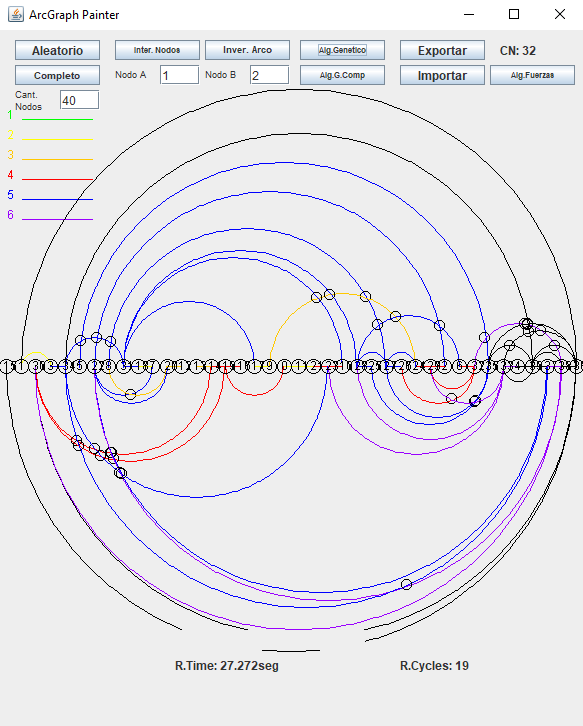
\includegraphics[width=0.45\textwidth]{imagenes/grafo_example_ori_gen.png}
	}
	\subfigure[Grafo luego de aplicar algoritmo dirigido por fuerzas de Tunkelang (CN: 34).]{
		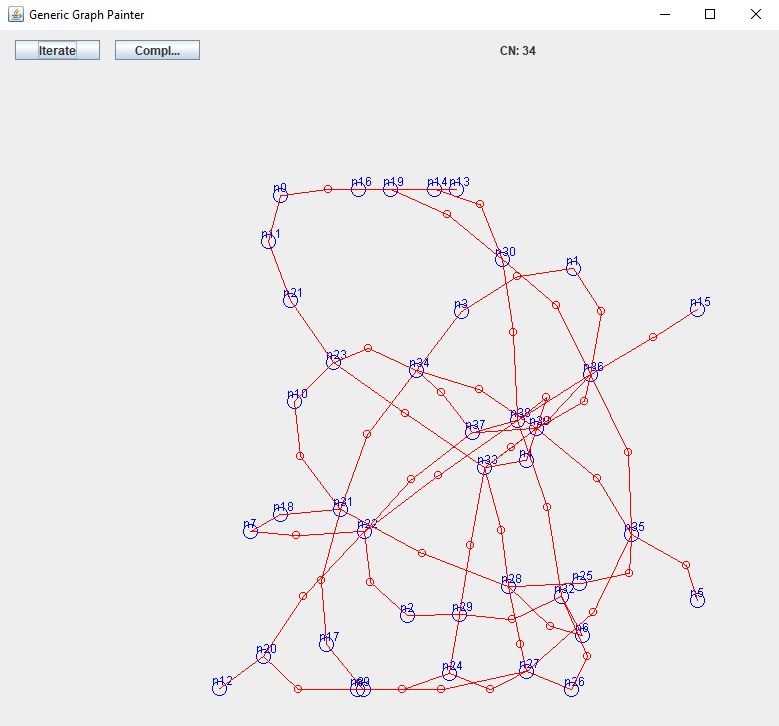
\includegraphics[width=0.5\textwidth]{imagenes/grafo_example_ori_gen_fue.png}
	}
	\caption{Ejemplo de aplicar algoritmo dirigido por fuerzas de Tunkelang sobre un grafo de 40 nodos aleatorio preprocesado por el algoritmo ArcGen.}
	\label{fig:resultado_ejemplo_grafo_ori_gen_fue}
\end{figure*}

\begin{table}[H]
	\caption{Promedios de 100 pruebas sobre cada semilla (de 5 a 50), del algoritmo dirigido por fuerzas de Tunkelang sobre los grafos originales aleatorios preprocesados por el algoritmo ArcGen.}
	\label{tab:resultados_gen_alg_fue}
	\begin{tabularx}{\linewidth}{|p{1.5cm}|p{1.2cm}|p{1.5cm}|X|X|}
		\hline
		\multirow{2}{2cm}{\textbf{Nro. Nodos (semilla)}} & \multicolumn{4}{c|}{\textbf{Promedios}} \\
		\cline{2-5}
		& \textbf{Nro. Arcos} & \textbf{Tiempo} & \textbf{CN Grafo Preprocesado} & \textbf{CN Grafo Final} \\
		\hline
		10 & 13 & 2.577 s. & 0 & 0 \\
		\hline
		15 & 20 & 2.691 s. & 1 & 2 \\
		\hline
		20 & 28 & 3.166 s. & 4 & 5 \\
		\hline
		25 & 35 & 4.352 s. & 7 & 9 \\
		\hline
		30 & 43 & 13.511 s. & 12 & 15 \\
		\hline
		35 & 50 & 18.140 s. & 19 & 22 \\
		\hline
		40 & 58 & 18.464 s. & 27 & 27 \\
		\hline
		45 & 65 & 26.062 s. & 34 & 37 \\
		\hline
		50 & 73 & 48.312 s. & 43 & 46 \\
		\hline
	\end{tabularx}
\end{table}

\section{Resultados Finales}
\label{sec:resultados_finales}
Finalmente se realiza la prueba completa, utilizando sobre el grafo original, el algoritmo para grafos completos, seguido por el algoritmo ArcGen y finalmente el algoritmo dirigido por fuerzas de Tunkelang. En la figura \ref{fig:resultado_ejemplo_grafo_ori_lin_gen_fue} puede verse un ejemplo del resultado final de aplicar todos los algoritmos. En la Tabla \ref{tab:resultados_orig_alg_com_gen_fue} pueden verse los promedios de tiempos de ejecución y de los crossing number resultantes para cada semilla. Luego, en la Tabla \ref{tab:resultados_comparacion} se comparan los resultados obtenidos anteriormente por el algoritmo de fuerzas con los resultados de esta prueba.

\begin{figure*}[h]
	\centering
	\subfigure[Grafo original (CN: 209).]{
		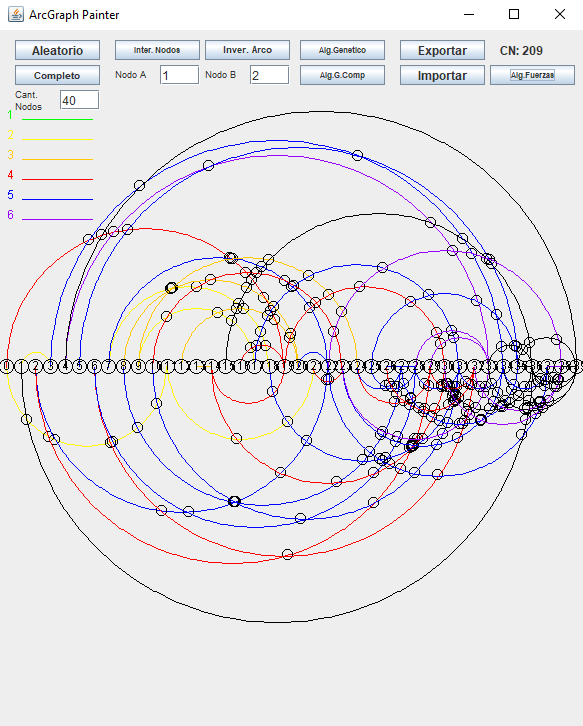
\includegraphics[width=0.45\textwidth]{imagenes/grafo_example_ori.png}
	}
	\subfigure[Grafo luego de aplicar el algoritmo para grafos completos, seguido del algoritmo ArcGen y finalmente el algoritmo dirigido por fuerzas de Tunkelang (CN: 34).]{
		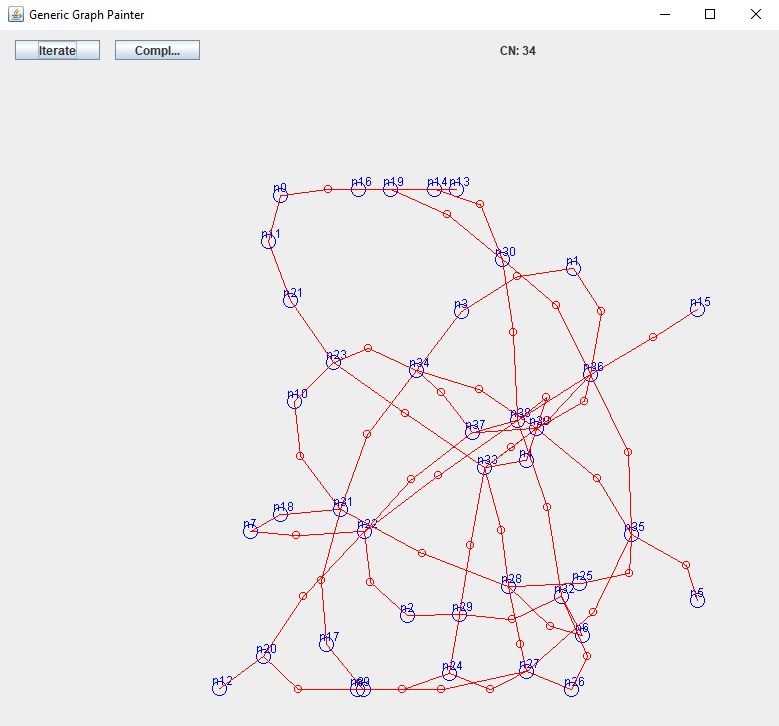
\includegraphics[width=0.5\textwidth]{imagenes/grafo_example_ori_gen_fue.png}
	}
	\caption{Ejemplo de aplicar algoritmo dirigido por fuerzas de Tunkelang sobre un grafo de 40 nodos aleatorio preprocesado por el algoritmo ArcGen y por algoritmo para grafos completos.}
	\label{fig:resultado_ejemplo_grafo_ori_lin_gen_fue}
\end{figure*}

%La Tabla \ref{tab:resultados_exp}\ presenta los promedios mencionados de los resultados recopilados de las ejecuciones del algoritmo genético sobre grafos generados en forma aleatoria, con diferentes cantidades de nodos. 

%	 La recopilación de resultados de ejecuciones del algoritmo genético sobre grafos generados aleatoriamente con diferentes cantidades de nodos y de estos se han obtenido promedios. Esta muestra los promedios de $100$ ejecuciones para cada número de nodos.


%Procesador sobre el que se corre.\\
%En general  trabajamos con modelos conceptuales que no tienen normalmente más de 4 arcos(relaciones entre los  nodos) por nodo (nodos conceptos o  clases o entidades)  

%Tenemos probablemente muchas clases (nodos)\\

%Teniendo en cuenta que la motivación del desarrollo de este algoritmo de layout es su incorporación y utilización en herramientas gráficas de modelado conceptual  y que generalmente los modelos no contienen  grandes cantidades de nodos, los test realizados sobre la aplicación  se han limitado a un máximo de 50 nodos.
\begin{table}[H]
	\caption{Promedios de 100 pruebas sobre cada semilla (de 5 a 50), del algoritmo dirigido por fuerzas de Tunkelang sobre los grafos originales aleatorios preprocesados, primero por el algoritmo para grafos completos y luego por el algoritmo ArcGen.}
	\label{tab:resultados_orig_alg_com_gen_fue}
	\begin{tabularx}{\linewidth}{|p{1.5cm}|p{1.2cm}|p{1.5cm}|p{1.5cm}|X|X|}
		\hline
		\multirow{2}{2cm}{\textbf{Nro. Nodos (semilla)}} & \multicolumn{5}{c|}{\textbf{Promedios}} \\
		\cline{2-6} & \textbf{Nro. Arcos} & \textbf{Tiempo} & \textbf{Ciclos} & \textbf{CN Inicial} & \textbf{CN Final} \\
		\hline
		10 & 13 & 2.556 s. & 2 & 7 & 0 \\
		\hline
		15 & 20 & 2.551 s. & 4 & 18 & 2 \\
		\hline
		20 & 28 & 2.625 s. & 6 & 38 & 5 \\
		\hline
		25 & 35 & 2.849 s. & 9 & 66 & 9 \\
		\hline
		30 & 43 & 4.326 s. & 12 & 103 & 15 \\
		\hline
		35 & 50 & 5.333 s. & 14 & 139 & 21 \\
		\hline
		40 & 58 & 5.745 s. & 18 & 195 & 28 \\
		\hline
		45 & 65 & 8.678 s. & 21 & 240 & 36 \\
		\hline
		50 & 73 & 13.414 s. & 25 & 312 & 44 \\
		\hline
	\end{tabularx}
\end{table}

\definecolor{green}{RGB}{0, 150, 0}

\begin{table}[H]
	\caption{Comparación de resultados finales de la pruebas realizadas. Los mejores resultados fueron marcados en \textbf{negrita}. En el caso de los tiempos se consideran el mismo si se aproximan en $\pm1$ segundo.}
	\label{tab:resultados_comparacion}
	\begin{tabularx}{\linewidth}{|X|X|X|X|X|X|X|X|}
		\hline
		\multirow{3}{2cm}{\textbf{Nro. Nodos (semilla)}} & \multicolumn{7}{c|}{\textbf{Promedios}} \\
        \cline{2-8} & \multirow{2}{2cm}{\textbf{Nro. Arcos}} & \multicolumn{3}{c|}{\textbf{Tiempos D.Fuerzas sobre}} & \multicolumn{3}{c|}{\textbf{CN Final D.Fuerzas sobre}} \\
		\cline{3-8} & & \textbf{Original} & \textbf{G.Comp.} & \textbf{ArcGen} & \textbf{Original} & \textbf{G.Comp.} & \textbf{ArcGen} \\
		\hline
		10 & 13 & \textbf{2.555 s.} & \textbf{2.557 s.} & \textbf{2.556 s.} & {1} & \textbf{0} & \textbf{0} \\
		\hline
		15 & 20 & \textbf{2.525 s.} & \textbf{2.527 s.} & \textbf{2.551 s.} & {3} & \textbf{2} & \textbf{2} \\
		\hline
		20 & 28 & \textbf{2.539 s.} & \textbf{2.537 s.} & \textbf{2.625 s.} & {6} & {6} & \textbf{5} \\
		\hline
		25 & 35 & \textbf{2.546 s.} & \textbf{2.545 s.} & \textbf{2.849 s.} & {10} & {10} & \textbf{9} \\
		\hline
		30 & 43 & \textbf{2.588 s.} & \textbf{2.589 s.} & {4.326 s.} & {17} & {17} & \textbf{15} \\
		\hline
		35 & 50 & \textbf{2.593 s.} & \textbf{2.593 s.} & {5.333 s.} & {24} & {23} & \textbf{21} \\
		\hline
		40 & 58 & \textbf{2.541 s.} & \textbf{2.543 s.} & {5.745 s.} & {32} & {31} & \textbf{28} \\
		\hline
		45 & 65 & \textbf{2.527 s.} & \textbf{2.527 s.} & {8.678 s.} & {42} & {41} & \textbf{36} \\
		\hline
		50 & 73 & \textbf{2.531 s.} & \textbf{2.536 s.} & {13.414 s.} & {52} & {51} & \textbf{44} \\
		\hline
	\end{tabularx}
\end{table}

%Los resultados obtenidos fueron aceptables respecto a lo esperado, en comparación con los algoritmos mencionados en el trabajo \cite{gibson2013survey}. La técnica Dirigida por Fuerzas de Tunkelang \cite{tunkelang1998jiggle},  una de las adecuadas, sufre de altos tiempos de ejecución y no promete un grafo óptimo,  según \cite{gibson2013survey}. \textsc{ArcGen} produce grafos con menores cruces a coste de un tiempo similar a la técnica Dirigida por Fuerzas, para los casos que se buscan resolver. En este sentido, estos resultados preliminares prometen un uso eficaz para fines prácticos de la futura herramienta finalizada.

%Como se puede observar en grafos con mayor cantidad de nodos y arcos,  {\sc ArcGen} disminuyó la cantidad de cruces en hasta cuatro veces.

% podemos encontrar que los algoritmos y técnicas de layout automático no presentan implementaciones libres que puedan ser utilizadas eficazmente en modelado conceptual. 